\subsubsection{Module MD-07: Quản lý Giao hàng (POS - Delivery)}
Module Quản lý Giao hàng (MD-07) là một thành phần quan trọng của hệ thống Point of Sale (POS), được thiết kế đặc biệt để hỗ trợ nhà hàng quản lý các đơn hàng mà khách yêu cầu giao đến một địa chỉ cụ thể. Module này tập trung vào việc thu thập thông tin khách hàng và địa chỉ giao hàng, xử lý đơn hàng, và đặc biệt là tích hợp với dịch vụ quản lý giao hàng của bên thứ ba (trong trường hợp này là Shipday) để tự động hóa việc gửi yêu cầu giao hàng và theo dõi trạng thái.



\begin{figure}[H]
    \centering
    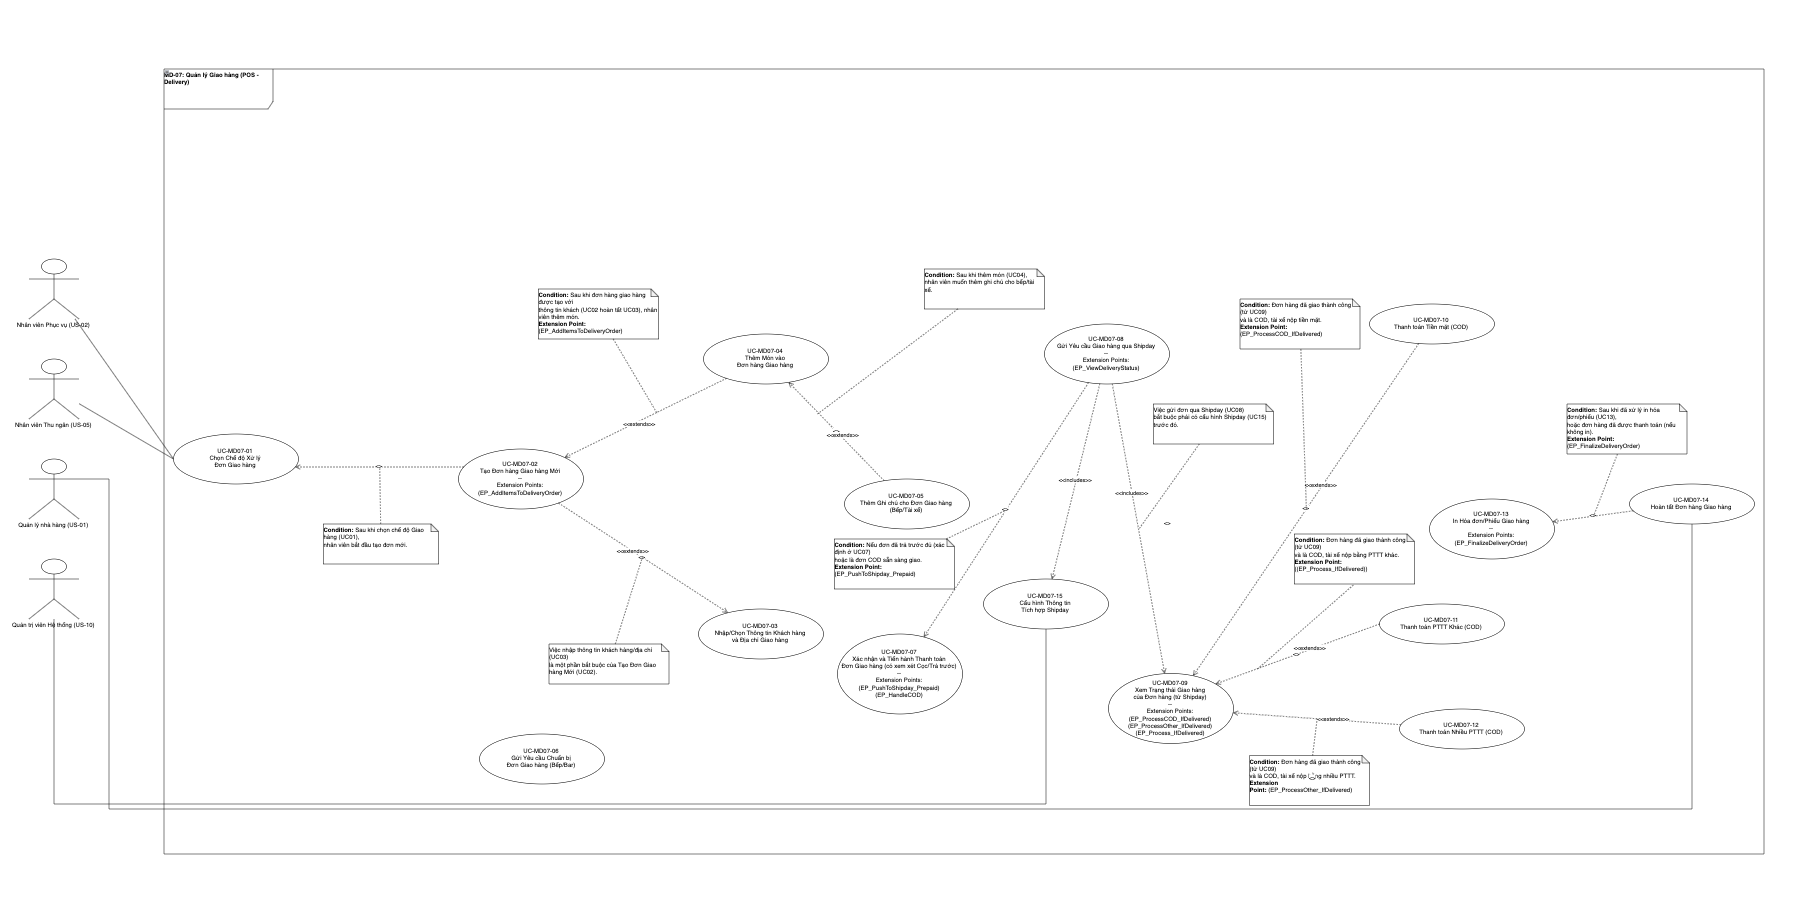
\includegraphics[width=15cm]{Sections/tong_quan/functional_spec/img/uc7.png}
    \vspace{0.5cm}
    \caption{Use case diagram cho Module MD-07}
    \label{fig:my_label}
\end{figure}

\begin{longtable}{|m{2cm}|m{2.5cm}|m{2.5cm}|m{4.5cm}|m{4cm}|}
\caption{Danh sách Yêu cầu Chức năng cho Module MD-07: Quản lý Giao hàng (POS - Delivery)} \label{tab:fr_md07_revised_v2} \\
\hline
\textbf{Mã Module} & \textbf{Mã Yêu cầu CN} & \textbf{Mã Người dùng} & \textbf{Tên Chức năng} & \textbf{Mô tả Ngắn} \\
\hline
\endhead % Header cho các trang tiếp theo
\hline
\endfoot % Footer cho bảng
\hline
\endlastfoot % Footer cho trang cuối cùng

MD-07 & FR-MD07-01 & US-02, US-05 & Chọn Chế độ Xử lý Đơn Giao hàng & Nhân viên chọn chế độ/giao diện riêng trên POS cho đơn giao hàng. \\
\hline
MD-07 & FR-MD07-02 & US-02, US-05 & Tạo Đơn hàng Giao hàng Mới & Nhân viên khởi tạo đơn hàng mới, yêu cầu liên kết thông tin khách hàng giao hàng. \\
\hline
MD-07 & FR-MD07-03 & US-02, US-05 & Nhập/Chọn Thông tin Khách hàng và Địa chỉ Giao hàng & Nhân viên tìm/chọn khách hàng có sẵn hoặc nhập mới Tên, SĐT, Địa chỉ giao hàng chi tiết. \\
\hline
MD-07 & FR-MD07-04 & US-02, US-05 & Thêm Món vào Đơn hàng Giao hàng & Nhân viên thêm món ăn/đồ uống vào đơn hàng giao đi. \\
\hline
MD-07 & FR-MD07-05 & US-02, US-05 & Thêm Ghi chú cho Đơn Giao hàng (Bếp/Tài xế) & Nhân viên thêm ghi chú cho bếp hoặc ghi chú cho tài xế giao hàng. \\
\hline
MD-07 & FR-MD07-06 & US-02, US-05 & Gửi Yêu cầu Chuẩn bị Đơn Giao hàng (Bếp/Bar) & Nhân viên gửi thông tin món cần chuẩn bị xuống bếp/bar, có đánh dấu "Delivery". \\
\hline
MD-07 & FR-MD07-07 & US-02, US-05 & Xác nhận và Tiến hành Thanh toán Đơn Giao hàng (có xem xét Cọc/Trả trước) & Nhân viên vào màn hình thanh toán, nơi hệ thống đã tự động áp dụng cọc/trả trước (nếu đơn hàng được đặt online và có trả trước). \\
\hline
MD-07 & FR-MD07-08 & US-02, US-05 & Gửi Yêu cầu Giao hàng qua Shipday & Sau khi đơn hàng sẵn sàng, nhân viên kích hoạt gửi thông tin đơn hàng sang Shipday. \\
\hline
MD-07 & FR-MD07-09 & US-02, US-05, US-01 & Xem Trạng thái Giao hàng của Đơn hàng (từ Shipday) & Nhân viên xem trạng thái giao hàng (Đã gán tài xế, Đang giao...) được cập nhật từ Shipday trên chi tiết đơn hàng. \\
\hline
MD-07 & FR-MD07-10 & US-02, US-05 & Thực hiện Thanh toán Tiền mặt cho Đơn Giao hàng (Nếu COD) & Nhân viên nhận tiền mặt COD từ tài xế và ghi nhận vào hệ thống. \\
\hline
MD-07 & FR-MD07-11 & US-02, US-05 & Ghi nhận Thanh toán bằng Phương thức Khác (Không Thẻ) cho Đơn Giao hàng (Nếu COD) & Nhân viên ghi nhận thanh toán COD bằng phương thức khác được hỗ trợ. \\
\hline
MD-07 & FR-MD07-12 & US-02, US-05 & Thực hiện Thanh toán Đơn Giao hàng bằng Nhiều Phương thức (Không Thẻ, Nếu COD) & Nhân viên nhận thanh toán COD bằng nhiều phương thức. \\
\hline
MD-07 & FR-MD07-13 & US-02, US-05 & In Hóa đơn/Phiếu Giao hàng & Nhân viên in hóa đơn/phiếu giao hàng để tài xế sử dụng. \\
\hline
MD-07 & FR-MD07-14 & US-02, US-05 & Hoàn tất Đơn hàng Giao hàng & Nhân viên đóng đơn hàng giao đi sau khi đã giao thành công và (nếu COD) đã nhận đủ thanh toán. \\
\hline
MD-07 & FR-MD07-15 & US-01/US-10 & Cấu hình Thông tin Tích hợp Shipday & Quản trị viên/Quản lý cấu hình các tham số kết nối API và Shipday. \\
\hline

\end{longtable}


\subsubsubsection{Mục tiêu và Phạm vi}
\label{sssec:md07_objectives_scope}
Mục tiêu chính của module MD-07 bao gồm:
\begin{itemize}
    \item \textbf{Quản lý hiệu quả đơn hàng giao đi:} Cung cấp một quy trình đầy đủ từ việc nhận đơn, nhập thông tin khách hàng và địa chỉ, xử lý món ăn, cho đến khi gửi đơn cho đơn vị vận chuyển và theo dõi.
    \item \textbf{Tích hợp liền mạch với dịch vụ giao hàng bên ngoài (Shipday):} Tự động hóa việc gửi thông tin đơn hàng sang Shipday để tìm tài xế và quản lý quá trình giao hàng.
    \item \textbf{Theo dõi trạng thái giao hàng:} Cập nhật trạng thái đơn hàng trong hệ thống dựa trên thông tin phản hồi từ Shipday.
    \item \textbf{Xử lý thanh toán linh hoạt cho đơn giao hàng:} Hỗ trợ các hình thức thanh toán như trả trước online hoặc thu tiền khi nhận hàng (COD).
    \item \textbf{Cung cấp thông tin chính xác cho các bên liên quan:} Đảm bảo bếp/bar nhận đúng yêu cầu chuẩn bị, tài xế có đủ thông tin giao hàng, và nhân viên nhà hàng có thể theo dõi quá trình.
    \item \textbf{Nâng cao trải nghiệm khách hàng:} Thông qua việc giao hàng đúng hẹn và thông tin rõ ràng.
\end{itemize}
Phạm vi của module bao gồm từ việc nhân viên chọn chế độ xử lý đơn giao hàng, tạo đơn hàng, nhập thông tin chi tiết, gửi yêu cầu chuẩn bị, gửi đơn sang Shipday, theo dõi trạng thái, cho đến khi xử lý thanh toán COD (nếu có) và hoàn tất đơn hàng.

\subsubsubsection{Đối tượng Sử dụng Chính}
\label{sssec:md07_primary_users}
Các đối tượng người dùng và hệ thống chính tương tác với module này bao gồm:
\begin{itemize}
    \item \textbf{US-02 (Nhân viên phục vụ) / US-05 (Nhân viên thu ngân):} Là những người trực tiếp nhận yêu cầu đặt hàng giao đi, tạo đơn hàng trên POS, nhập thông tin khách hàng, địa chỉ, món ăn, và gửi yêu cầu giao hàng sang Shipday.
    \item \textbf{US-01 (Quản lý nhà hàng):} Có thể thực hiện tất cả các chức năng của nhân viên, giám sát quá trình, xử lý các trường hợp đặc biệt, và cấu hình tích hợp.
    \item \textbf{US-10 (Quản trị viên Hệ thống):} Chịu trách nhiệm cấu hình kỹ thuật cho việc tích hợp API với Shipday.
    \item \textbf{System (Hệ thống Shipday):} Hệ thống tự động hóa nhiều bước, trong khi Shipday là hệ thống bên ngoài chịu trách nhiệm quản lý đội xe và quá trình giao hàng thực tế.
\end{itemize}

\subsubsubsection{Các Chức năng Chính}
\label{sssec:md07_key_functionalities}
Module MD-07 cung cấp một chuỗi các chức năng để quản lý toàn diện quy trình giao hàng, được mô tả chi tiết qua các Use Case sau:

\begin{itemize}
    \item \textbf{Khởi tạo và Chuẩn bị Đơn hàng Giao hàng (UC-MD07-01 đến UC-MD07-06):}
    \begin{itemize}
        \item Cho phép nhân viên chọn chế độ hoạt động hoặc giao diện dành riêng cho việc xử lý đơn hàng giao đi (UC-MD07-01).
        \item Nhân viên khởi tạo một đơn hàng POS mới, được hệ thống tự động đánh dấu là loại hình "Giao hàng" (UC-MD07-02).
        \item Yêu cầu nhân viên bắt buộc phải nhập hoặc chọn thông tin khách hàng và địa chỉ giao hàng chi tiết cho đơn hàng (UC-MD07-03).
        \item Thêm các món ăn/đồ uống từ thực đơn POS vào đơn hàng giao đi (UC-MD07-04, tương tự UC-MD05-05).
        \item Thêm các ghi chú đặc biệt cho bếp (về món ăn) hoặc cho tài xế (về việc giao hàng) (UC-MD07-05, tương tự UC-MD05-07 nhưng có thêm ghi chú cho tài xế).
        \item Gửi thông tin các món cần chuẩn bị của đơn hàng giao đi xuống các máy in bếp/bar hoặc màn hình KDS, có chỉ dẫn rõ là đơn "Delivery" (UC-MD07-06, tương tự UC-MD05-08 nhưng có thêm thông tin "Delivery").
    \end{itemize}

    \item \textbf{Xử lý Thanh toán và Tích hợp Giao hàng (UC-MD07-07, UC-MD07-08, UC-MD07-10, UC-MD07-11, UC-MD07-12):}
    \begin{itemize}
        \item Trước khi vào màn hình thanh toán hoặc xác nhận đơn, hệ thống tự động kiểm tra và áp dụng (trừ đi) các khoản tiền đặt cọc hoặc thanh toán trước (nếu có) cho đơn hàng giao đi (UC-MD07-07).
        \item Gửi thông tin chi tiết của đơn hàng (bao gồm địa chỉ, thông tin khách, món ăn, số tiền COD nếu có) đến hệ thống quản lý giao hàng Shipday thông qua API (UC-MD07-08).
        \item Đối với đơn hàng COD, cho phép nhân viên ghi nhận việc đã nhận tiền mặt từ tài xế (UC-MD07-10, tương tự UC-MD05-12).
        \item Ghi nhận việc tài xế nộp tiền COD bằng các phương thức khác tiền mặt (ví dụ: chuyển khoản) (UC-MD07-11, tương tự UC-MD06-09 cho Takeout).
        \item (Tùy chọn) Ghi nhận việc tài xế nộp tiền COD bằng nhiều phương thức kết hợp (UC-MD07-12, tương tự UC-MD05-14).
    \end{itemize}

    \item \textbf{Theo dõi và Hoàn tất Đơn hàng Giao hàng (UC-MD07-09, UC-MD07-13, UC-MD07-14):}
    \begin{itemize}
        \item Hiển thị trạng thái giao hàng mới nhất của đơn hàng (ví dụ: "Đang giao", "Đã giao thành công") được hệ thống tự động cập nhật từ Shipday (thường qua webhook) (UC-MD07-09).
        \item In hóa đơn hoặc phiếu giao hàng chi tiết cho đơn hàng giao đi, để đính kèm gói hàng hoặc giao cho khách (UC-MD07-13, tương tự UC-MD06-11).
        \item Chính thức đóng đơn hàng giao đi trong hệ thống sau khi đã xác nhận giao hàng thành công và tất cả các vấn đề thanh toán đã được xử lý (UC-MD07-14, tương tự UC-MD06-12).
    \end{itemize}

    \item \textbf{Cấu hình Tích hợp (UC-MD07-15):}
    \begin{itemize}
        \item Cho phép Quản lý/Quản trị viên thiết lập và quản lý các tham số cần thiết để kết nối và trao đổi dữ liệu với nền tảng Shipday, bao gồm API Key (UC-MD07-15).
    \end{itemize}
\end{itemize}

\subsubsubsection{Tóm tắt Luồng Hoạt động Tổng thể}
\label{sssec:md07_overall_workflow}
Luồng hoạt động chính trong module Quản lý Giao hàng (POS - Delivery) thường diễn ra như sau:
\begin{enumerate}
    \item \textbf{Cấu hình ban đầu:} Quản lý/Quản trị viên Cấu hình Thông tin Tích hợp Shipday (UC-MD07-15).
    \item \textbf{Nhận và tạo đơn hàng giao đi:}
        \begin{itemize}
            \item Nhân viên Chọn Chế độ Xử lý Đơn Giao hàng (UC-MD07-01).
            \item Hệ thống yêu cầu, và nhân viên Tạo Đơn hàng Giao hàng Mới kèm theo việc Nhập/Chọn Thông tin Khách hàng và Địa chỉ Giao hàng (UC-MD07-02, UC-MD07-03).
            \item Nhân viên Thêm Món vào Đơn hàng Giao hàng (UC-MD07-04) và Thêm Ghi chú cho Đơn Giao hàng (Bếp/Tài xế) (UC-MD07-05).
            \item Nhân viên Gửi Yêu cầu Chuẩn bị Đơn Giao hàng (Bếp/Bar) (UC-MD07-06).
        \end{itemize}
    \item \textbf{Xử lý thanh toán và gửi giao hàng:}
        \begin{itemize}
            \item Nhân viên tiến hành xác nhận đơn, hệ thống tự động xem xét và áp dụng các khoản Cọc/Trả trước (UC-MD07-07).
            \item Sau khi đơn hàng sẵn sàng (đã chuẩn bị, thông tin thanh toán rõ ràng), nhân viên Gửi Yêu cầu Giao hàng qua Shipday (UC-MD07-08).
        \end{itemize}
    \item \textbf{Theo dõi và hoàn tất:}
        \begin{itemize}
            \item Nhân viên có thể Xem Trạng thái Giao hàng của Đơn hàng (từ Shipday) (UC-MD07-09) được cập nhật tự động.
            \item Khi cần, nhân viên In Hóa đơn/Phiếu Giao hàng (UC-MD07-13).
            \item Nếu là đơn COD và đã giao thành công, nhân viên ghi nhận thanh toán từ tài xế: Tiền mặt (UC-MD07-10), Phương thức Khác (UC-MD07-11), hoặc Nhiều Phương thức (UC-MD07-12).
            \item Cuối cùng, sau khi giao thành công và thanh toán hoàn tất, nhân viên hoặc hệ thống Hoàn tất Đơn hàng Giao hàng (UC-MD07-14).
        \end{itemize}
\end{enumerate}
Module MD-07 kết hợp các chức năng POS nội bộ với khả năng tích hợp mạnh mẽ của Shipday, tạo nên một giải pháp toàn diện cho việc quản lý dịch vụ giao hàng của nhà hàng.

